\section{Solving Subinstances}
In this section, we discuss the implementation of the different approaches to
solving several subinstances.
As mentioned in the beginning of the chapter, the two
main approaches are to solve a limited amount of subinstances, bounded
by some $s$, or to implement a discrete event simulator that only stores
the current state of the network. First we will discuss the implementation
of the tree structure, before we move on to the two main approaches.

\subsection{Tree Structure}
All trees consists of vertices, and in our specific case, each vertex contains
two sets $\mathcal{M}$ and $\mathcal{Z}$, a solution $x^*$, and a number of
child vertices. To keep vertices as simple as possible, we implement them as
simple \texttt{structs}. Each vertex \texttt{struct} looks like
this:
\begin{verbatim}
struct vertex {
    std::set<uint16_t> m;
    std::set<uint16_t> z;
    double* sol;
    std::vector<struct vertex*> children;
};
\end{verbatim}
A reader familiar with \texttt{C++} might notice that we use
\texttt{std::set} instead of using a bit vector as we discussed
in Chapter \ref{ch:tree}, and we will come to that later. Note that
the sets consist of indices of primitive type \texttt{uint16\_t}, which is
short for \texttt{unsigned short int}. That means that the sets are limited to
$2^{16} = 65536$ elements, and therefore also putting a limit to the size
of the QP problems that can be solved. This seems like a reasonable limit
as GoodTech wants to solve problems with $200 - 2000$ variables.
If they need to solve larger problems in the future, it is possible to change
the primitive data type.

As soon as a vertex is defined, we are ready to implement \texttt{mfind}.
Remember that \texttt{mfind} is a modified version of \texttt{find} that tells
us which vertex should be the parent of our potentially new vertex in case it
has a distinct solution.
\texttt{mfind} is defined in two parts. The first part is a ''helper'' function
for starting the algorithm on some vertex. The second part is the actual
recursively defined algorithm. These two parts are called \texttt{mfind} and
\texttt{mfindrec}, respectively. We define \texttt{mfind} as follows:
\newpage
\begin{verbatim}
struct vertex* mfind(const std::set<uint16_t>&m,
const struct vertex* v, bool& found) {
    found = true;
    if (isSubset(v->m, m) && isSubset(m, v->z)) return v;
    found = false;
    return mfindrec(m, v, found, v);
}
\end{verbatim}
The parameters for \texttt{mfind} are a modifier, a vertex where the search
will begin and a boolean value that will tell us whether we found a
solution or not.
In order to search the whole tree, one would use the root vertex as parameter
\texttt{v}. The function returns a pointer to a vertex of our interest.
Note that this is a pointer, and not an index like in Algorithm
\ref{alg:mfind}. The function makes a call to \texttt{mfindrec}:
\begin{verbatim}
struct vertex* mfindrec(const std::set<uint16_t>& m,
const struct vertex* v, bool& found, struct vertex* ret) {
    for (struct vertex* vi : v->children) {
        if (isSubset(vi->m, m) {
            ret = vi;
            if (isSubset(m, vi->z)) {
                found = true;
                return vi;
            } else mfindrec(m, vi, found, ret);
        }
    }
    return ret;
}
\end{verbatim}
It is quite evident from the code that the performance of the \texttt{isSubset}
function is important. In Chapter \ref{ch:tree} we discussed using bit vectors 
to represent sets. We concluded that a simple \texttt{AND} operation would tell
us whether a set was a subset of another set.
We also discussed the possibility of it being more memory efficient than
storing sets in a sparse format where only the indices of each variable was
stored.

Using a bit vector, each set consumes exactly $n$ bits of storage if our
\emph{universe} holds $n$ variables.
Using sets of sparsely stored indices, each set consumes a varying amount of
bits depending on how many variables are in the set. If each index is of data
type \texttt{uint16\_t}, then each index consumes $16$ bits. The trade-off
here is quite clear: If a set contains less than one sixteenth of $n$, then
the sparse format uses less memory. This might actually be the case in a lot
of sets, especially when solving all possible subinstances where the number
of breakdowns are limited by some $b$. Consider a very small case where
$n = 200$ and we solve all sub instances $s = \sum_{j=0}^{3} {200 \choose j}$.
With a total number of $s$ sets stored as bit vectors, the memory use for
storing the modifiers is $200s~\textrm{bits} \approx 32~\textrm{megabytes}$.
Whereas, with $s$ sets of sparsely stored indices, the memory use for storing
the modifiers is approximately $8$ megabytes. However, the more $b$ increases,
the greater the benefits of storing sets in bit vectors become evident. As soon
as $b$ becomes greater than 12, bit vectors will use less memory to store all
modifiers. Figure \ref{fig:bmem} shows the ratio of memory used by bit vectors
over memory used by sets of sparsely stored indices where $n = 200$ and
$5 \leq b \leq 30$.
\begin{figure}[h!]
\begin{center}
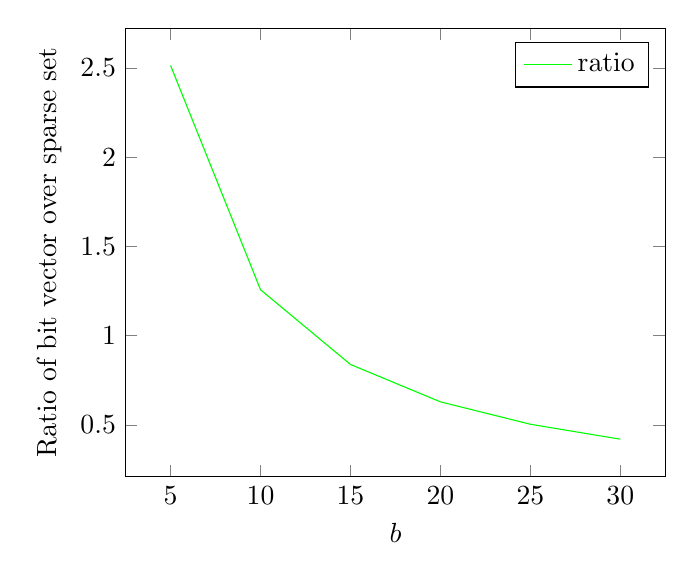
\begin{tikzpicture}
    \begin{axis}[
        legend pos=north east,
        xlabel=$b$,
        ylabel=Ratio of bit vector over sparse set]

        \addplot[green] plot coordinates {
            (5,  2.51302)
            (10, 1.25686)
            (15, 0.838169)
            (20, 0.628847)
            (25, 0.503276)
            (30, 0.419585)
        };

        \legend{ratio}
    \end{axis}
\end{tikzpicture}
\end{center}
\caption{Difference in memory use with bit vectors and sparse sets.}
\label{fig:bmem}
\end{figure}
Aside from the modifier set, we also have to store the set of variables that
are equal to zero in the optimal solutions of each subinstance. These sets
are more difficult to analyze in terms of memory use, simply because the
cardinality is unknown. However, we do know that $|\mathcal{Z}_i| \geq
|\mathcal{M}_i|$ for $i=1,2,\ldots,n$.

With sets of sparsely stored indices, we only need to check the variables
that are actually in the sets in order to determine if a set is a subset
of some set. However, with bit vectors, we need to check $n$ bits---where $n$
is the number of variables in the universe---in order to determine the same.


\newpage
\begin{comment}
struct vertex* findrec(const std::set<uint16_t>& m, struct vertex* v) {
    for (int i = 0; i < v->children.size(); i++) {
        struct vertex* child = v->children[i];
        if (isSubset(child->m, m) {
            if (isSubset(m, child->z))
                return child;
            else
                findrec(m, child);
        }
    }
    return 0;
}
The function \texttt{isSubset} is just a one-line function that calls
\texttt{std::includes(...)}. One might notice that we do not check if the input
vertex contains the solution to the input modifier. However, we \emph{do} check
this in \texttt{find}:
struct vertex* find(const std::set<uint16_t>& m, struct vertex* v) {
    if (v == 0) return 0;
    if (isSubset(v->m, m) && isSubset(m, v->z) return v;
    return findrec(m, v);
}
\end{comment}
